The training data consists of a subset of the LibriSpeech dataset \cite{panayotov_librispeech_2015} which is processed according to the pipeline shown in figure \ref{fig:data_pipeline}. In total, the dataset consists of 2255 speech utterances, 35 impulse responses, and 20 noise recordings. In order to avoid overfitting, each time a speech file is loaded, it is randomly cropped, then paired with a segment of a randomly chosen noise file and a randomly chosen impulse response. In the data pipeline presented, noise is added before the convolution takes place. This is done in an effort to model real rooms where ambient noises are also convolved with the reverberation of the room. This ordering is important to note, as most approaches use the reverse ordering.	It is also important to note that the result of the convolution operation is truncated to retain the same length as the target signal. This is necessary so that the loss function can be easily be computed between the network output and the target.

\begin{figure}[h]
	\centering
	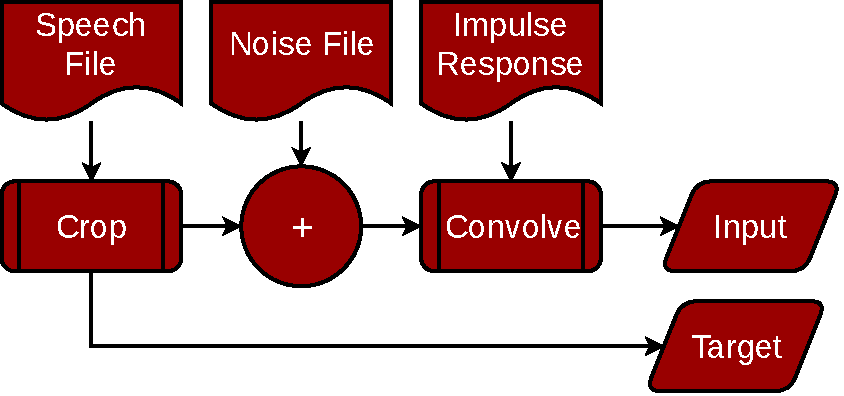
\includegraphics[width=0.5\textwidth]{data_pipeline}
	\caption{Data pipeline}
	\label{fig:data_pipeline}
\end{figure}
